%The internal structure, describing the relevant data need for AllSpark in
%order to reach its goals, can be resumed in this list:
%\begin{itemize}
%\item {\bf Employee:} Allspark has some different kind of employees, 
%they are divided mainly into Developers, Sysadmins, Analysts and Administration
%staff.
%\item {\bf Suppliers:} Our organization has to rely on different suppliers as
%Hardware supplier, Software Supplier and Connectivity supplier.
%\item {\bf Project:} The projects in which AllSpark is involved, are divided
%in two categories, Security System or Service hosting.
%\item {\bf Customer:} Another kind of useful data is the collection of our 
%customer with relative contracts.
%\item {\bf Partner:} AllSpark works in collaboration with organization of 
%various kind, they can be Universities, Opensource Foundations and external 
%consultants.
%\end{itemize}
%
%The class diagram in figure \ref{img:data2} can describe more efficently
%the main data on which aur organization works.
%
\begin{figure}[!ht]
\centering
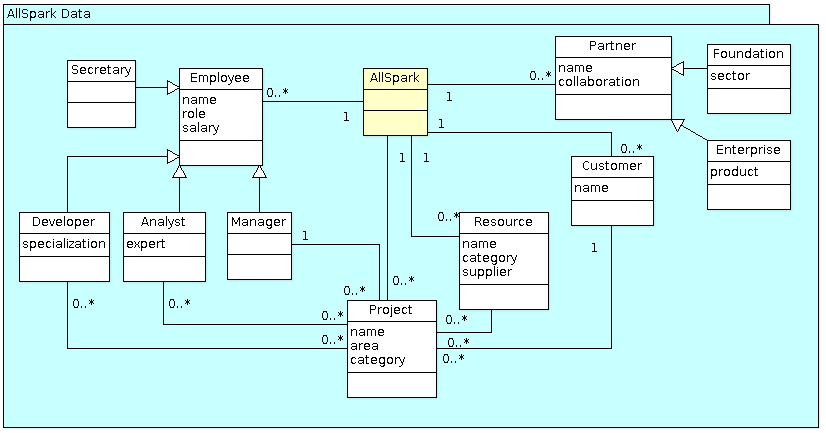
\includegraphics[scale=0.63,angle=90]{argouml_diags/imgs/data2}
\caption{Class diagram representing the relevant internal data}
\label{img:data2}
\end{figure}
